
%%% Local Variables:
%%% mode: latex
%%% TeX-master: t
%%% End:

% !Mode:: "TeX:UTF-8"

\chapter{基于任务精确预测的实时功耗温度管理}
\label{cha:DPTM}

\section{实时系统的工作负载模型}
\label{sec:workload}
本文讨论的实时系统的工作负载模型具有简单的结构。 系统会周期性地分配一段时间$D$,某一任务的必须在该截止时间以前完成。该任务在最坏情况下所需要的执行时间为$W$。 本文中假设任务的截止时间等于系统周期性分配的时间片,并且等价地只考虑一个周期内任务的执行情况。 根据任务的性质,\onlinecite{RTCalSchHdRTSys}与\onlinecite{LkSchMaxTemMinPerHdRTSys}等文献研究了如何估计$(D,W)$数据对的值。
本文中我们认为工作负荷是发送至实时系统的网络流量的归一化形式。


\section{实时系统的热分析模型}
\label{sec:thermal}
为了研究处理器内核(Die)的热传导特性, 文献\onlinecite{LkDVSRTEmbSys,LkSchMaxTemMinPerHdRTSys,WCTemAnlyRTSys}等都广泛采用了等效RC电路方法进行热分析, 并采用式\ref{equ:chap2:thermal-model}进行内核工作温度的分析
\begin{equation}
\label{equ:chap2:thermal-model}
\frac{dT}{dt} = \frac{P}{C_{th}}-\frac{T-T_{amb}}{R_{th}C_{th}} = \alpha P -\beta (T-T_{amb})
\end{equation}
式\ref{equ:chap2:thermal-model}中$T$和$T_{amb}$分别代表芯片的温度与环境温度, $P$代表芯片在时刻$t$的功耗,$R_{th}$与$C_{th}$分别为等效热阻与等效热容。

\section{实时系统的功耗分析模型}
\label{sec:power}
多数处理器拥有两种主要模式,即工作状态和休眠状态:只有在工作状态下处理器被充足供电,并执行计算任务; 否则,处理器将进入休眠状态以减少功耗,同时降低自身温度。工作状态下的功耗为:
\begin{equation}
\label{equ:chap2:active-power}
P_{active} = CV_{dd}^2f+N_{gate}I_{leakage}V_{dd}
\end{equation}
式\ref{equ:chap2:active-power}中的第一项代表动态功耗,第二项代表静态功耗。当给定供电电压$V_{dd}$后,工作频率$f$为
\begin{equation}
\label{equ:chap2:freq}
f = \frac{(V_{dd}-V_t)^\mu}{(V_{dd}T_{max})^\eta}\times 4.2824\times 10^{14} \approx C_1V_{dd}
\end{equation}
由于与工作电压成正比,我们可以使用式\ref{equ:chap2:active-power-simplified}计算动态功耗
\begin{equation}
\label{equ:chap2:active-power-simplified}
P_{active} = C_2V_{dd}^3
\end{equation}
通过HSPICE软件进行的曲线拟合,与温度、电压相关的漏电流可写为
\begin{equation}
\label{equ:chap2:leakage-current}
I_{leakage} = I(V_0,T_0)(AT^2\exp(\frac{\alpha V_{dd}+\beta}{T})+B\exp(\gamma V_{dd}+\delta))
\end{equation}
式\ref{equ:chap2:leakage-current}中$A,B,\alpha,\beta,\gamma,\delta,\mu,\eta$是经验参数,由芯片的生产工艺参数所决定。 本文的模拟实验默认选择采用65nm的工艺参数,具体参数数值见表\ref{tab:chap2:tech-parameters}。
\begin{table}
\caption{$A,B,\alpha,\beta,\gamma,\delta,\mu,\eta$的取值}
\centering
\begin{tabular}{c c c c c c c c c}
\hline\hline
参数 & $A$ & $B$ & $\alpha$ & $\beta$ & $\gamma$ & $\delta$ & $\mu$ & $\eta$ \\
\hline
取值 & 1.143E-12 & 1.013E-14 & 466.403 & -1224.741 & 6.282 & 6.909 & 1.19 & 1.20 \\
\hline
\end{tabular}
\label{tab:chap2:tech-parameters}
\end{table}

当工作温度$T$在300K到380K的正常范围变化时,$\exp(\frac{1}{T})$的波动变化很小。 当给定了$V_{dd}$后, 文献\onlinecite{EngRTTskSchTemDepLk}通过引入两个参考温度$TH$和$TL$进一步将漏电流简化为温度的二次函数。 于是,与漏电流相关的静态功耗可以用式\ref{equ:chap2:leakage-power}计算
\begin{equation}
\label{equ:chap2:leakage-power}
P_{leakage} = N_{gate}(\hat{A}T^2+\hat{B})V_{dd}
\end{equation}
\ref{equ:chap2:leakage-power}中,
$\hat{A}=\frac{I_{leakage}(TH,V_{dd})-I_{leakage}(TL,V_{dd})}{{TH}^2-{TL}^2}$,
$\hat{B}=I_{leakage}(TH,V_{dd})-\hat{A}{TL}^2$。
此外,处理器在两种工作状态之间的切换是通过改变工作电压来实现的, 状态切换将带来额外的开销,包括能耗开销$p_r$与延时开销$c_r$\onlinecite{TemIdDistEngOptDVS}。 整体而言,工作状态切换跨度越大(切换电压差越大),其能耗和时间的开销也就越大。

\section{目前流行的动态温度与功耗调度策略}
\label{sec:algorithms}
\subsection{考虑漏电流的温度敏感技术(简称TALk技术)}
Gang Qu\onlinecite{TemLkMinTechRTSys,DPTMbyYJQ}提出的考虑漏电流的温度敏感技术技术根据工作负载和截止时间的不同, 来控制不同时间段处理器的工作/休息状态:当负载量大并且温度较低时、处理器处于激活工作状态; 当负载量小并且温度较高时,处理器切换到睡眼状态以减小能耗,以降低温度。
具体而言,该算法会实时监测两个重要的调度指标。其一是当前工作负载量和剩余空闲时间的比例$\eta$, 其二是将芯片调至睡眠状态下的温度下降速率与将芯片调至工作状态下的温度上升速率的比例$\theta$。 如果前者大于后者,说明当前处理器的任务负载较重,同时即便让芯片休息,降温的效率也不会高,于是算法判定让处理器继续执行任务; 而如果前者小于后者说明任务较轻,休息状态降温效率高,便将处理器就处于休息状态,降低芯片温度,同时节约芯片的静态功耗。 其中$\eta$比较直观且容易计算,而$\theta$则较为复杂。首先,要计算处理器当前的工作温度$T_{current}$, 而后要分别计算该芯片在工作和睡眠状态下的稳定温度$K_1,K_2$(即经过了无穷长时间后的温度), 最后用式\ref{equ:chap2:cal-theta-talk}计算得到速率比值。
\begin{equation}
\label{equ:chap2:cal-theta-talk}
\theta=\frac{T_{current}-K_2}{K_1-T_{current}}
\end{equation}



\subsection{基于固定周期的技术(简称Pattern-Based,PB技术)}

基于固定周期的算法将任务的截止时间或者运行周期D等分为n个时间片段,每段长$\Delta=D/n$, 采用PB算法的处理器将工作于特定规则的模式中\onlinecite{EngRTTskSchTemDepLk,DPTMbyYJQ}: 执行$\Delta=D/n$时间后便切入休眠模式,以减少功耗并降低温度。 文献\onlinecite{EngRTTskSchTemDepLk}与\onlinecite{WCTemAnlyRTSys}证明:如果重复这种运行模式足够多次, 处理器将达到温度的平衡值,并进入稳定状态, 即每个周期的初始温度和结束温度将趋向于稳定值,以便于分析。

\subsection{M阶震荡调节技术(简称M-Oscillating,MO技术)}

上面介绍的TALk算法和PB算法都要求处理器的工作速度要大于或者等于负载率$W/D$。 具有DVS或者DVFS功能的实时性系统往往只允许芯片可以工作在几个电压档上,并可以根据负载率调节实际处于的电压值。 这就会导致芯片一直工作在高于需求的速度上。这不仅增加了动态功耗和静态功耗(因为他们分别是电压的三次方和一次方函数),还 会加速温度的上升,提高平衡温度的值,最终导致漏电流以二次方的速度增长。一种显而易见的解决方法是允许处理器在两个不同速度下工作。 文献\onlinecite{LkSchMaxTemMinPerHdRTSys}证明,如果采用两个最接近的速度完成分配给处理器的任务, 那么相对于采用其他的工作速度组合, 处于该速度组下处理器的温度是最优的。 如果进一步地将这种两步策略应用在m个时间片中\onlinecite{DPTMbyYJQ}, 不仅温度可以进一步优化,还可以将$D$时间内的总功耗表达为$m$的函数, 而且必然存在能耗最小化的$m$值\onlinecite{LkEngMinRTSysMaxTemConst}。 由于要考虑电压切换所付出的时间开销和能耗开销,\onlinecite{LkEngMinRTSysMaxTemConst}给出了$m$所具有确定的 上限值$Ceil$。

\subsection{小结与评价}
作为温敏调度算法,TALk参照剩余任务量与当前温度、来合理地调度任务。 然而,简单的开关模式无法利用DVS技术,只能工作在固定速度。而且状态切换所导致的时间、能耗开销也是不可避免的。 根据切换时间和能耗开销\onlinecite{TemIdDistEngOptDVS},从全速工作转变为零电压将产生最大的能耗和时间开销。

无论采用TALk还是PB算法,都要求处理器工作在大于$W/D$的速度上。 大多数具有DVS或DVFS功能的实时系统通常只允许芯片的电压为若干离散值,根据负载率来调整电压工作档。 这往往会导致芯片实际上工作高于任务所需的速度,不仅增加了近似与电压三次方成正比的动态功耗和与电压近似成正比的 静态功耗, 而且加速了温度的攀升, 抬高了平衡态时的温度,进一步导致漏电流近似平方速度的增长。

G.Quan等\onlinecite{LkEngMinRTSysMaxTemConst}提出的MO算法也存在两个主要缺陷。首先,假设功率为温度的线性函数, 使得峰值温度较PB有很大降低。 其次是在实际应用中不能忽略低工作负载率情况:当$W/D$小于处理器支持的最低工作速度时,MO只能退化为PB, 以防止不必要的功耗增加。

\section{基于电压预测的温敏漏电流技术(简称VP-TALk技术)}
\begin{figure}[H] % use float package if you want it here
  \centering
  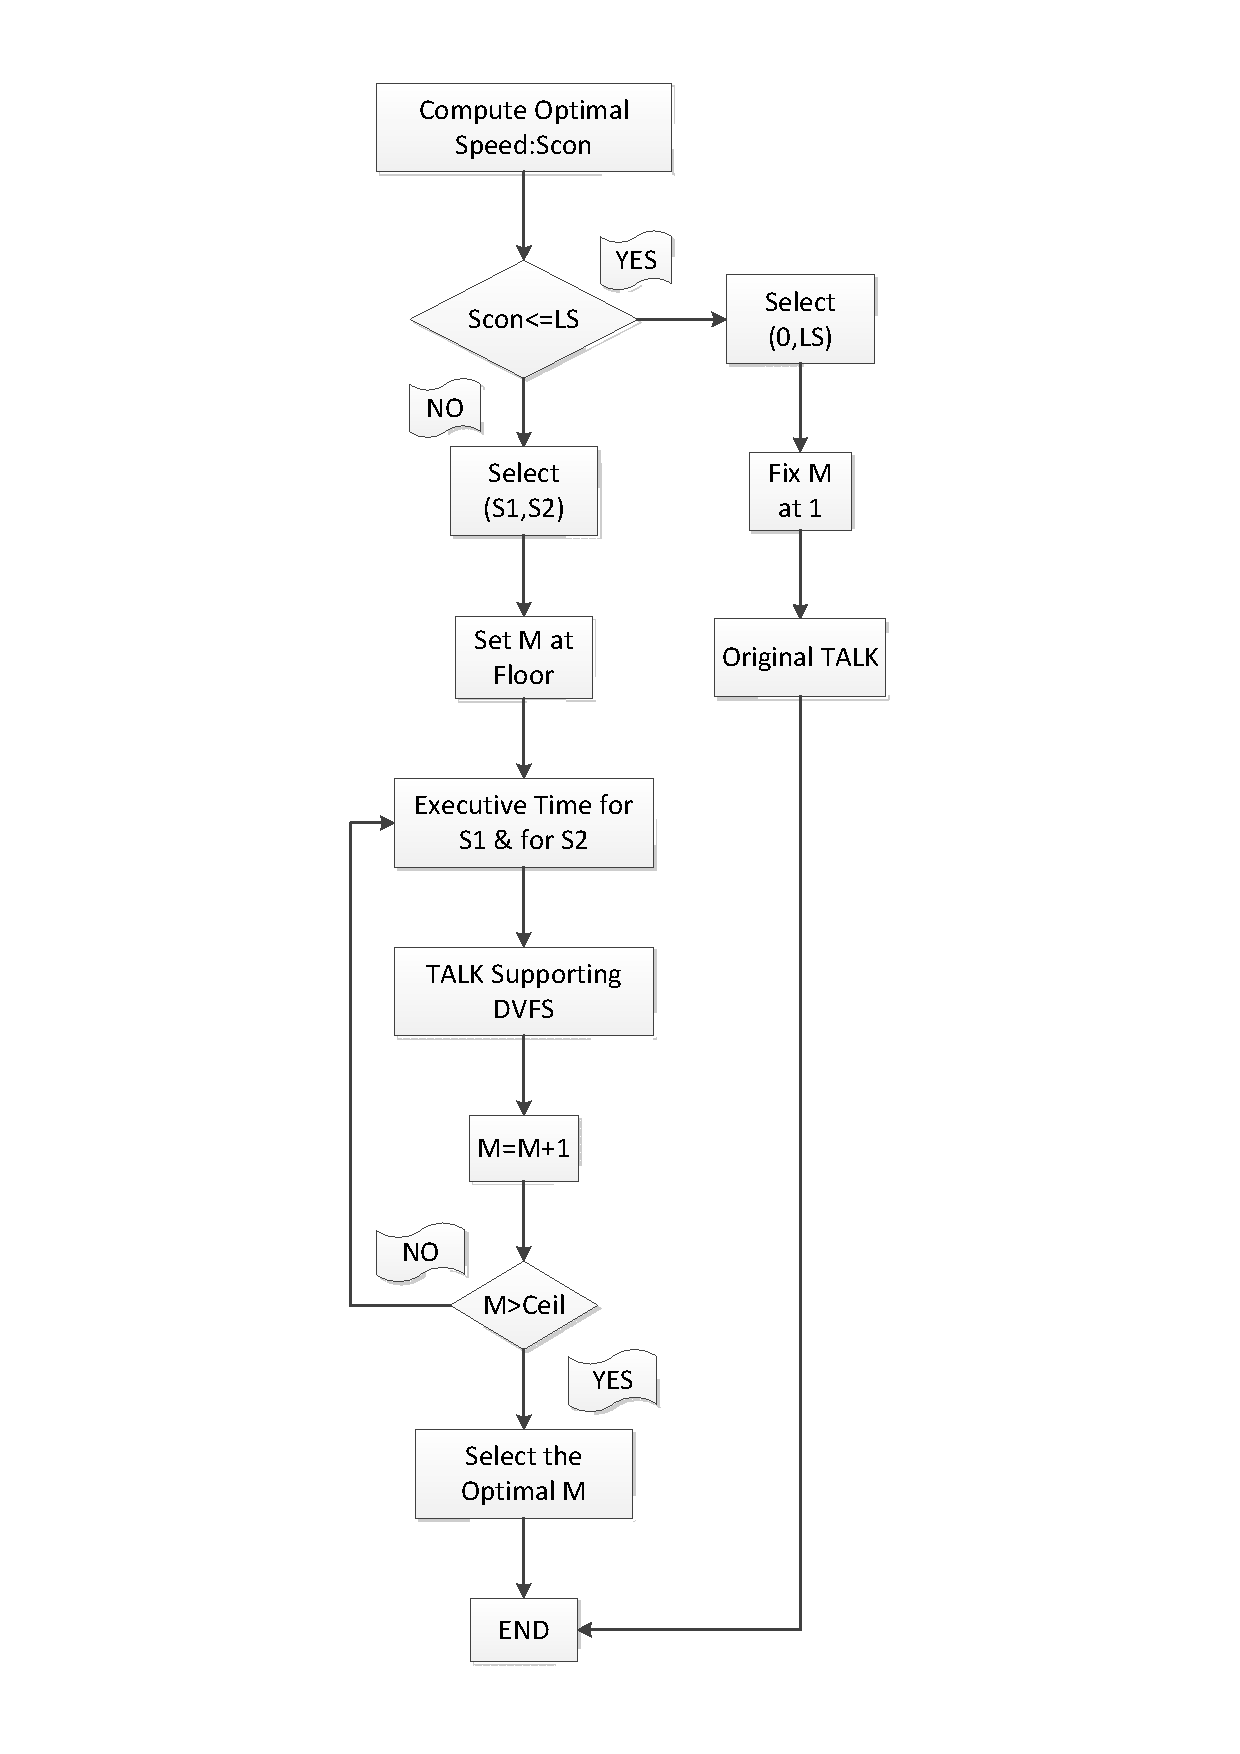
\includegraphics[width=0.8\textwidth,height=0.8\textheight]{Visio-VS-TALK}
  \caption{基于电压预测的温敏漏电流技术的流程图}
  \label{fig:vp-talk}
\end{figure}
\label{sec:vp-talk}
根据我们在DPTM领域的研究经验,可以获得如下关于DPTM改进的几点经验准则:
\begin{enumerate}[1)]
\item 必须考虑温度对静态功耗的影响。本文将功耗定为温度的二次函数。在温度限制下,DPTM系统最好具有温敏调控功能。
\item 如果能够准确预测负载量,确定任务所需的工作频率或者工作电压,就可以提前调度,更好的满足实时性。
\item 芯片电压选取。由于工作电压决定了运行速度,应该采用MO的电压选取方法,即使得芯片运行速度刚好满足工作负载的需求, 以最大程度地利用DVFS技术来降低能耗。
\item 调度过程中,必须考虑电压切换(状态切换)所带来的额外能耗、时间开销。
\end{enumerate}

基于以上观察,我们提出一种改良后的TALk算法,即具有电压选择的TALk算法,本文称为VP-TALk, 其算法流程图如图\ref{fig:vp-talk}所示。

与MO相似,VP-TALk首先需要假设电压可以连续调节、以获得理论上的最优工作速度$S_{con}$。在$S_{con}\leq LS$(芯片最低工作速度)时, VP-TALk等同于原始的TALk算法。在$S_{con}>{LS}$时,该算法选用两档邻接的速度$S_1$和$S_2$,使得$S_1\leq S_{con}<S_2$。 不同于MO的等分$M$段时间段,VP-TALk采用更灵活的、电压可调的温敏TALk来对每一小段的工作状态进行调度,即对每一个小的时间片, 采用TALk中定义的两个调度指标($\eta$与$\theta$)来决定是将芯片设置为休眠或是工作状态。 由于$m$的数量由切换工作状态的代价和任务的实时性所限制, 其上下限分别记为$Ceil$和$Floor$,计算方法可仿照\onlinecite{LkEngMinRTSysMaxTemConst}中的方法。 VP-TALk的应用前提是假设我们已经通过某种预测的方法预测出了任务负载量,从而,在任务到达前调度就已经开始,所以认为是实时性的。

\section{动态温度与功耗管理系统}
\label{DPTM-system}
\subsection{启发性示例}
在之前的分析中,我们已经指出,较轻工作负载时的MO必然要退化至PB的方法. 这是因为当工作所需电压低于可选的最小电压值时,MO中阶梯型工作电压策略无法通过逼近最优工作电压的方式节省动态功耗。 为了探究工作量与最优调度算法之间的关系,我们设定任务长度为10秒, 并考虑比文献\onlinecite{LkEngMinRTSysMaxTemConst}更强的温度对漏电流影响, 我们在工作负载率全区间(5\%-95\%)范围内,对TALk、PB与MO这3种已有调度源算法的调度效果进行了考察。 图\ref{fig:exp-power-cmp}给出了能耗的数据,图\ref{fig:exp-temp-cmp}给出了温度数据。
\begin{figure}%[H] % use float package if you want it here
  \centering
  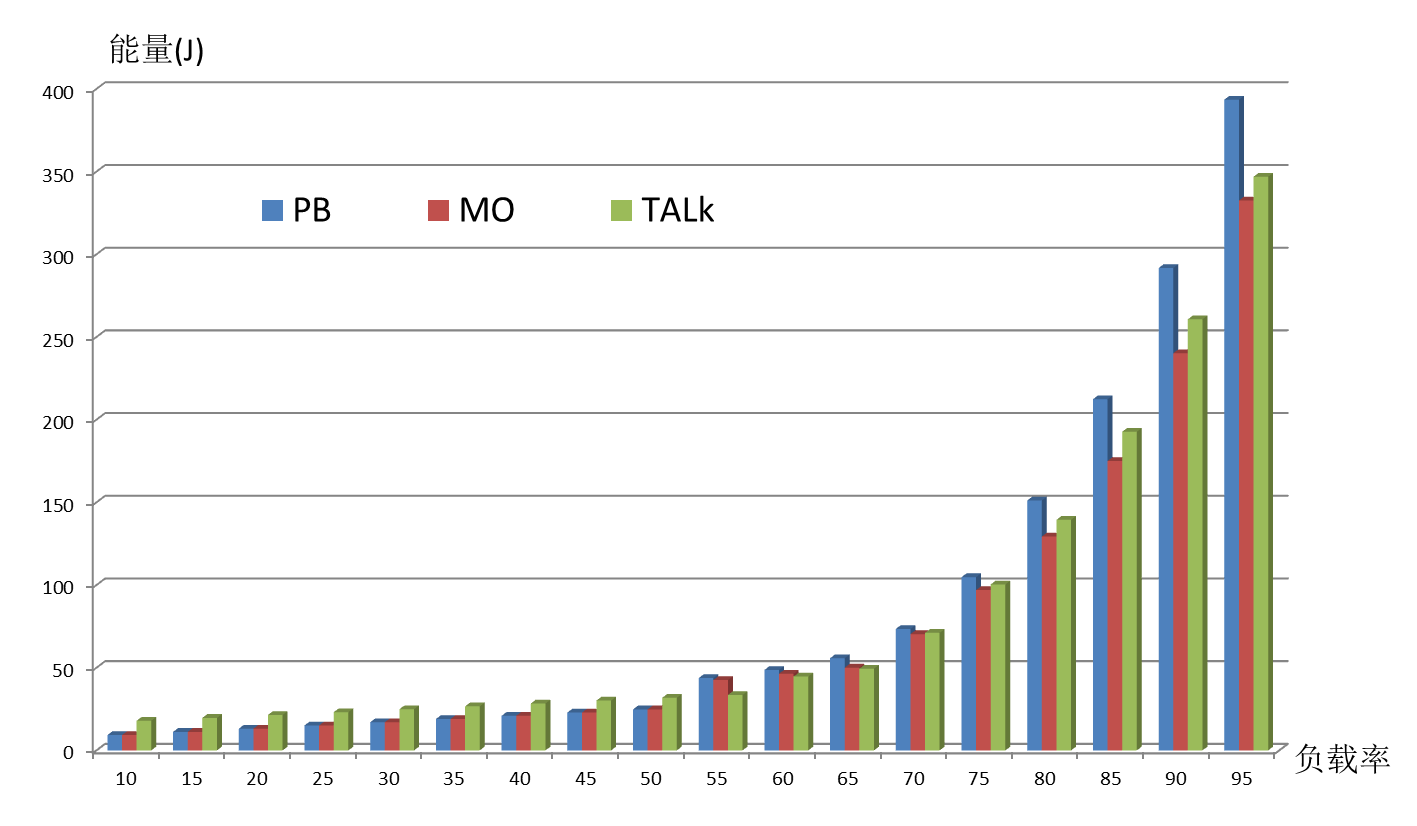
\includegraphics[width=1.0\textwidth]{POWER-CMP}
  \caption{各种调度算法的能耗效果随负载率变化的比较}
  \label{fig:exp-power-cmp}
\end{figure}
\begin{figure}%[H] % use float package if you want it here
  \centering
  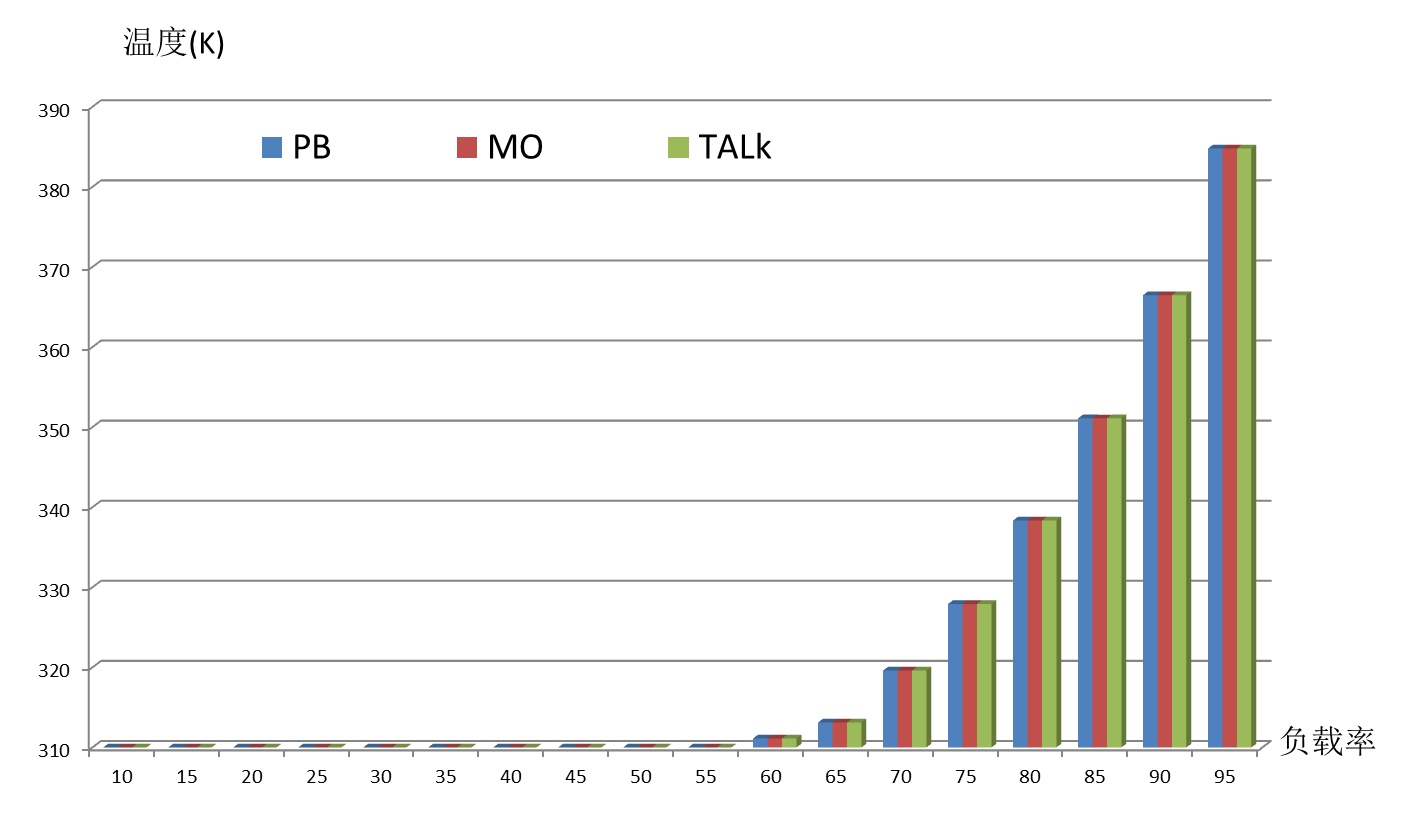
\includegraphics[width=1.0\textwidth]{TEMP-CMP}
  \caption{各种调度算法的峰值温度效果随负载率变化的比较}
  \label{fig:exp-temp-cmp}
\end{figure}

我们可以得出如下结论:
\begin{enumerate}[1)]
\item 当工作负载率($W/D$)低于50\%(近似值)时,三种源算法的峰值温度低于310K(37\celsius), 峰值温度对系统的性能与可靠性没有影响;在系统能耗方面,PB算法(也即MO算法)的调度效果要胜过TALk算法, 因此,PB算法具有最佳的调度效果。
\item 当工作负载率($W/D$)处于50\%-70\%区段(近似值)时,三种源算法的峰值温度低于320K(47\celsius), 峰值温度对系统的性能与可靠性也没有影响;在系统能耗方面,TALk算法的调度效果要胜过PB和MO算法, 因此,TALk算法具有最佳的调度效果。
\item 当工作负载率($W/D$)大于70\%(近似值)时,三种源算法的峰值温度高于320K(47\celsius ),最高可超过380K(107\celsius ),峰值温度对系统的性能与可靠性具有明显影响,其中MO算法具有最低的峰值温度;在系统能耗方面, MO算法的调度效果要明显胜过其它两种源算法,MO算法具有最佳的调度效果。
\end{enumerate}

由此可见,最优的DPTM调度算法与工作负载率有直接关系。我们将以此关系作为理论基础,用于DPTM调度原型系统的构建, 即根据对实时系统工作负荷的精确预测结果,来选择效果最佳的调度算法,并对DPTM调度效果进行评价。

\subsection{基于时间序列分析的工作负载预测}
\label{sec:prediction}
本文采用文献\onlinecite{DPTMbyYJQ}中所提出的基于时间序列分析的工作负载预测模型来满足VP-TALk算法预知工作负载率的需求。 大量的模拟实验已经证明, \onlinecite{DPTMbyYJQ}所提出的组合预测模型可以得到平均相对误差低于3\%、归一化方差小于0.5的任务负载预测效果。 具体的负载预测模型构建的公式推导和演化请参见本人已发表的\onlinecite{DPTMbyYJQ}的相关章节。这里,主要简单介绍整个预测流程。
实时系统的任务从其本质属性来讲,可以分为三种不同的成分。本文认为,工作负载$X(t)$中包含
\begin{enumerate}[1)]
\item 趋势成分$T(t)$:对应任务量随着时间而平稳增长、衰减的性质;
\item 周期成分$P(t)$,对应任务量随时间变化表现出的规律性;
\item 随机成分$R(t)$,对应任务量之中不确定的随机性。
\end{enumerate}
从而可以将任务看作三者之和:$X(t)=T(t)+P(t)+R(T)$。基于对三种基本成分的分析,本文提出了基于灰色模型、 傅里叶级数分解模型以及径向基函数(RBF)人工神经网络理论的组合预测数学模型,根据若干数量的真实的任务负载历史数据, 预测片上系统下一个时间步的近似任务量。具体而言,
\begin{enumerate}[1)]
\item 趋势成分反映工作负载随着时间演变而增加或衰减的趋势。为了弱化随机扰动因素的影响, 灰度模型GM(1,1)模型\onlinecite{GMModelGrayModel}通过累加原始数据数列, 发现该序列的指数增长规律;
\item 对于一个周期函数,最成熟的分析方法就是用傅里叶级数展开或者傅里叶变换;
\item 众所周知,任何服务系统的工作任务都会有一定的随机性,称之为任务负载中的随机成分。径向基函数神经网络是通过非线性基函数的线性组合, 对非线性函数关系具有良好的逼近能力,适于描述网络流量的复杂因素,如非线性、时变性等, 并可克服BP神经网络训练时间长及计算复杂度高的不足\onlinecite{RGSJWLSFYJYY}。
\end{enumerate}

\subsection{基于在线评价的动态温度与功耗管理系统}
根据调度算法性能与工作负载大小相关的观察,以及基于时间序列分析的工作负载预测,我们提出了在线评价、选择DPTM调度算法的调度策略, 并以此构建了本文的实时功耗温度管理原型系统。整个系统由工作负载预测、调度策略选择和调度策略评价三大模块组成。
在该系统工作中,其三大模块主要完成如下功能。
\begin{enumerate}[1)]
\item 工作负载预测模块:我们根据负载变化周期的长短,提出了一种组合式的负载预测方法, 采用多种不同拟合方法来分别对任务的不同物理意义成分进行精确预测,以获得对复杂任务的精确预测;
\item 调度策略选择模块:我们综合考虑实时完成任务、温度上限、能耗最小化、 漏电流与温度相关以及芯片模式切换代价等多种因素, 选用不同的任务调度策略;
\item 调度策略评价模块:对每种策略的系统能耗与峰值温度进行评价,并将其作为实时功耗温度管理系统的反馈量,供调度策略选择模块参考。
\end{enumerate}

调度策略选择的学习主要通过后期性能评价的评价值完成。假设存在$N$类算法,编号为$1,2,……,N$。 它们在某一时刻$t$的得分或者权重为,$w_t=(w_{1t},w_{2t},...,w_{Nt})$对其中任一个权重分量$w_{kt}$可以 采用式\ref{equ:chap2:cal-weight}进行计算
\begin{equation}
\label{equ:chap2:cal-weight}
w_{kt} = 1- \sum\limits_{j=t_0}^{t-1} \frac{E_{k,j}\lambda_j}{\sum\limits_{i=1}^N E_{i,j}}
\end{equation}
式\ref{equ:chap2:cal-weight}中$E_{i,j}$代表芯片使用第$i$类DPTM算法在时刻$j$的负载情况下消耗的能量, $\lambda_{j}$为一可调整的参数, 代表时刻$j$的能耗情况对决策的影响程度,$t_0$是可以变动的初始值, 它的取值意味着选取从何时开始的能耗情况作为以后决策的参考。在预测出工作负荷值后, 则开始使用式\ref{equ:chap2:decide}进行决策:
\begin{equation}
\label{equ:chap2:decide}
DPTM_t = \arg(\max\limits_{1\le k \le N}(w_{k,t}))
\end{equation}
式\ref{equ:chap2:decide}中$DPTM_t$为$t$时刻选择出的动态功耗温度调度策略。考虑到温度上的限制, 我们需要考察所选的调度源算法是否会超过温度上限。 如果能耗的节约是在很高的峰值温度的代价下换取的,我们将放弃该源算法,而选择次优的但是有较低峰值温度的调度源算法。
与三种已有源算法和本文提出的VP-TALk算法相比,本文实时功耗温度管理系统的主要扩展改进点在于: 具有高精度的任务预测模块,为根据负载量而进行的策略选择提供前提基础; 通过基于调度效果评价的机器学习,自适应地根据负载量的轻重选择调度策略。

\subsection{基于单一调度策略的动态温度与功耗管理系统}
值得一提的是,如果我们选定某一种调度策略,省略机器学习模块,就构成了基于单一调度策略的实时功耗温度管理原型系统。 在该实时功耗温度管理原型系统中,输入量为任务负载的历史值,通过这些历史值,利用第\ref{sec:prediction}节所述的任务负载预测模型, 可以得到对于下一时刻任务量的预测值。 进而,可以确定完成预测任务值所需要的芯片电压或者频率,并利用上文所述的任意某一种算法进行调度。
